\section{Random Forests}

The Random Forest Algorithm is a commonly used one because of its ease of implementation and easily interpretable results. It differs from Principal Component Analysis in a few ways, but namely because it is a supervised learning algorithm. Random Forests “see” the response variable in a data set, whether that be some numerical value for regression problems or some categorical value for classification problems. In this way, Random Forests are similar to linear regression models. On the other hand, PCA is unsupervised, so the algorithm does not have access to the response variable (Donges, 2018). 

\subsection{Decision Trees}
To understand a Random Forest, one must first take a look at the Decision Tree algorithm. Recall that for a given data set, we have a number of features and one response variable for each entry. View a sample data set below for a classification problem predicting success or failure.

\begin{table}
\begin{center}
\begin{tabular}{| c | c | c | c | c |}
\hline
\textbf{Contest ID} & \textbf{Feature 1} & \textbf{Feature 2} & \dots & \textbf{Response} \\ 
\hline
1 & 5.3 & 1.9 & \dots & Success \\  
\hline
2 & 2.4 & 7.6 & \dots & Failure \\
\hline
\vdots & \vdots & \vdots & \ddots & \vdots \\
\hline
\end{tabular}
\end{center}
\end{table}

Now that we have explored the structure of the data that we will feed the Decision Tree algorithm, we can continue on to a visualization of that data that will aid in the explanation of its implementation. To simplify our example, we consider a two-dimensional dataset with two features and a categorical response variable. The data could appear as the plot below. 

\begin{center}
\begin{figure}[]
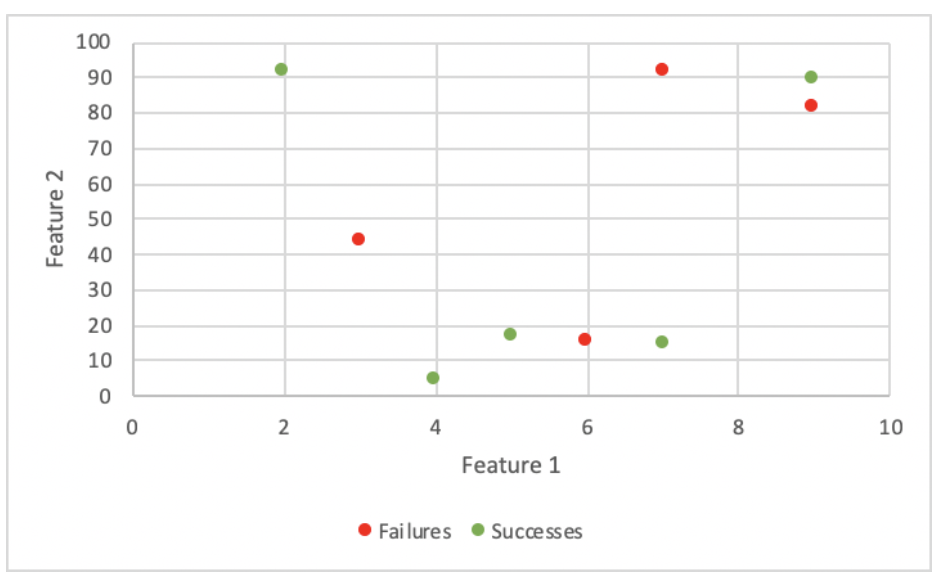
\includegraphics[width=8cm]{body/background/blanktree.png}
\end{figure}
\end{center}

Imagine a vertical or horizontal line in this two dimensional plot that separates the data points. Now we may predict that everything to the left of a vertical line is a success and everything to the right of the vertical line is a failure. Obviously, in our example above, any vertical line would have provide some error with this methodology. In other words, we predict that everything left of the line is a success, but indeed there are points left of that line which are categorized as failures. We could in this case test every vertical and horizontal line that changes how many data points are on either side. After doing so, we could choose the line with the smallest number of mislabeled points. The Decision Tree algorithm is recursive in that after that first line is drawn, another line may be drawn on the side of the first with the most error. We can repeat that process until there is only one point left in our region, as shown below. The associated decision tree can also be found in the figure below. 

\begin{center}
\begin{figure}[]
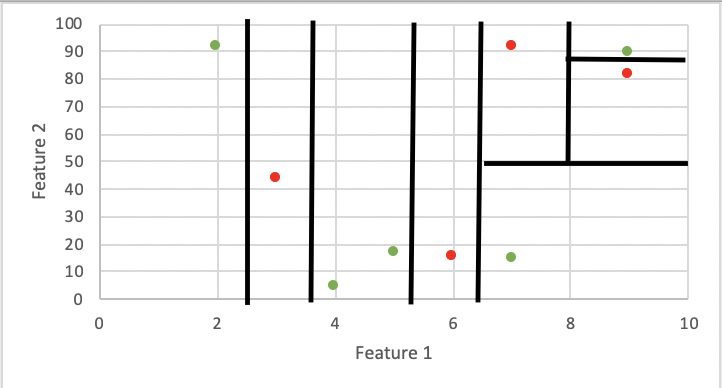
\includegraphics[width=8cm]{body/background/cuttree.png}
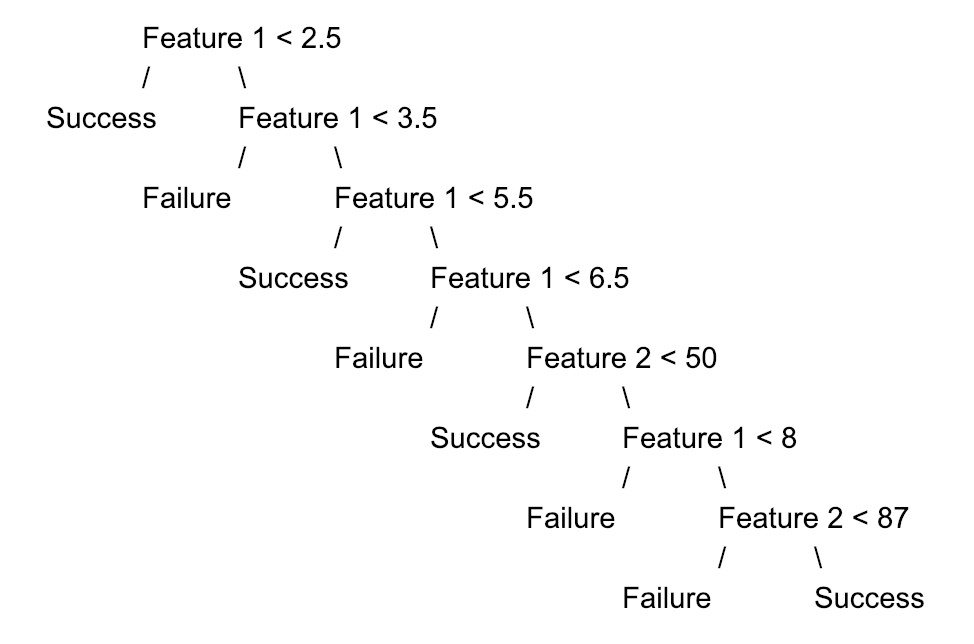
\includegraphics[width=8cm]{body/background/decisiontree.png}
\end{figure}
\end{center}

It is important to note in this model, at each branch, only one feature may be considered for categorization. During each iteration, we may only break along the axis of Feature 1 or the axis of Feature 2, and not along some diagonal dependent on both. This example is easily extended to the multidimensional case with more than two features, as the algorithm will first find the break along any feature axis that reduces the error in labeling, then continue on along the region with more errors. We can also use decision trees for regression problems, where we would predict a numerical response at each cut. For the purposes of this project, we need only consider the classification application. \newline

$\tab$ For each decision tree, certain parameters are fed into the model that can affect the final result. First, the number of features that a given decision tree receives can be tuned. A common practice is to give a decision tree approximately n features, where n is the total number of features. Secondly, we can limit the number of branches that a decision tree is allowed to make. In our previous example, we gave the tree free reign to divide the data until our remaining region contained only one point. When implementing the algorithm, we can tune this parameter to make each individual tree less accurate. This aspect is important to avoid overfitting. A decision tree that has all the features and can make as many branches as possible is likely to overfit, or build its predictions too closely off the training data. By varying which features each decision tree gets, how many branches it can make and then by averaging the results, the random forest is less likely to overfit than any given decision tree.  
\newline 

$\tab$ A Random Forest then, is a collection of a many decision trees generated along a typically random assortment of parameters. For example, we may run a random forest of 1000 decisions trees. We give each decision tree approximately n features, randomly selected from our n features. One hundred decision trees can make as many branches as necessary, one hundred can make 9 branches, one hundred can make 8, so forth down to one hundred that can make only 1 branch. This is a common implementation of the random forest algorithm. In this algorithm, each decision tree gets a “vote”, weighted equally in most cases, as to the categorization of each point. For example, if 950 of the 1000 decision trees in our random forest predict the point with ID 1 as a success, we would say that we are 95\% sure the point is truly a success (Paffenroth, 2018). \newline

\tab As far as training and testing procedure, we would typically divide the original data into training data and testing data with a 75/25 or 80/20 split. We would use the training data to build the random forest of decision trees with the lowest amount of error. Then, using the splits that these trees generate, we compare the testing data sorted via those branches to the actual success and failures, which we know because this is a supervised learning technique. Finally, we can generate a ROC curve or a confusion matrix to measure the accuracy of this model.

\subsection{Advantages and Disadvantages}
\tab One distinct advantage of random forests are their easy interpretability. For example, if the first cut was typically made along Feature 1, the user would know that Feature 1 is an important predictor for the response variable. Random forests are also easy to use and implement compared to other algorithms, and typically produce a good prediction result. However, a random forest does require a fair amount of computing time depending on how many trees it creates, so it can be costly to make real time predictions using this method. Lastly, random forests are typically used for predictive modeling, so it can be challenging to make inferences about the relationships between your variables using this method (Donges, 2018).

\subsection{Ensemble Learning}
\tab Linear Regression, Random Forests and Decision Trees can all be considered base models that could be used in Ensemble Learning. In fact, we would consider a Random Forest to be an ensemble of decision trees, each with different parameters. For a problem where prediction is the goal, we can utilize a number of different techniques together. This conglomerate of techniques has numerous predictions within, and when considered together, can give a more accurate prediction with less error than any one technique on its own. \newline

\tab An important methodology to implement ensemble learning is called bagging, or bootstrap aggregation. Bootstrapping is the process by which a random sample is taken from the data set for each model used in the ensemble. For example, if we had a data set with 1000 entries and wanted to build a random forest, we may take a random sample, with replacement, of 100 of those entries. In this case we assume that each sample is independently drawn and will represent the actual distribution of the whole set. This prevents the phenomenon of data snooping, or the act of using the same data twice in subsequent iterations of your model. After bootstrapping the data and feeding it to each model in the ensemble, the predictions are aggregated and we arrive at a final prediction for our testing data (Lutins, 2017; Paffenroth, 2018)
\newline \tab 

Errors are reduced in ensemble learning because of the nature of the collection. If a single model makes an error based on the limited data it has, that error can be easily corrected by numerous other models which have other data. In this way, by measure averages rather than single results, an ensemble can be more effective for predictive modeling than any one technique. Therefore, our team devised an ensemble of models to best tackle our problem. 